%!TEX program = xelatex

\documentclass{acm_proc_article-sp}

\usepackage{graphicx}
\usepackage{hyperref}

\begin{document}

\title{Evolutionary Algorithms for the Induction of Decision Trees}
%
% You need the command \numberofauthors to handle the 'placement
% and alignment' of the authors beneath the title.
%
% For aesthetic reasons, we recommend 'three authors at a time'
% i.e. three 'name/affiliation blocks' be placed beneath the title.
%
% NOTE: You are NOT restricted in how many 'rows' of
% "name/affiliations" may appear. We just ask that you restrict
% the number of 'columns' to three.
%
% Because of the available 'opening page real-estate'
% we ask you to refrain from putting more than six authors
% (two rows with three columns) beneath the article title.
% More than six makes the first-page appear very cluttered indeed.
%
% Use the \alignauthor commands to handle the names
% and affiliations for an 'aesthetic maximum' of six authors.
% Add names, affiliations, addresses for
% the seventh etc. author(s) as the argument for the
% \additionalauthors command.
% These 'additional authors' will be output/set for you
% without further effort on your part as the last section in
% the body of your article BEFORE References or any Appendices.

\numberofauthors{2} %  in this sample file, there are a *total*
% of EIGHT authors. SIX appear on the 'first-page' (for formatting
% reasons) and the remaining two appear in the \additionalauthors section.
%
\author{
% You can go ahead and credit any number of authors here,
% e.g. one 'row of three' or two rows (consisting of one row of three
% and a second row of one, two or three).
%
% The command \alignauthor (no curly braces needed) should
% precede each author name, affiliation/snail-mail address and
% e-mail address. Additionally, tag each line of
% affiliation/address with \affaddr, and tag the
% e-mail address with \email.
%
% 1st. author
\alignauthor
Ben Shulman\\
       \affaddr{Cornell University}\\
       \email{bgs53@cornell.edu}
% 2nd. author
\alignauthor
David Stauffer\\
       \affaddr{Cornell University}\\
       \email{dms483@cornell.edu}
}

\maketitle
\begin{abstract}
We show that evolutionary algorithms can be effectively used for decision tree induction. Decision tree induction is the creation of a tree which represents a function which takes an example with specific attributes and returns a label, or class, for the example. In this paper we show how  basic genetic algorithms for decision tree induction can outperform random trees as well as random forests along with baseline optimization algorithms such as random-mutation hillclimber and random search. We present a Pareto-based genetic algorithm which uses training error, tree size and tree age to induce decision trees that outperform standard greedy algorithms such as C4.5, as well as random forests, random mutation hillclimber and random search. Finally we provide a discussion of why age and size together can control for overfitting in Pareto-based strategies as well as tree simplicity and generalizability. We end this paper by discussing how our algorithms could be extended to potentially create more accurate and generalizable classifiers through co-evolution, and forests.
\end{abstract}

\section{Introduction}

Decision Trees are a data structure that describe a function that maps input examples to a label. Thus decision trees are a type of classifier. In particular at each node of the decision tree a comparison is made which compares an attribute of the example being classified. Depending on the result of that comparison the tree then makes another comparison or classifies the example. Thus the tree recursively sorts an example until a leaf is reached, at which point the example is classified. Nodes within the tree are comparisons while leafs are labels for examples.

One major class of machine learning algorithms are those that induct decision trees for a problem. These algorithms take a training set of examples, which have known labels, and constructs a decision tree (or trees) that performs well on the training set, with the idea that it will perform well on new un-seen examples. The most common method for creating decision trees is top-down induction of decision trees, which is a recursive greedy strategy. ID3 and C4.5 are examples of algorithms that generate trees in this way. In particular ID3 and C4.5 use information gain on the training set to select the best attribute to split on at each node, and then continues recursively to generate each subtree. Another example is random forests, which is a technique in which a set of a decision trees are created that then each label an example and the final label is determined by vote.

A problem with the traditional greedy algorithms is that greedy search leads them to search only a small area of the search space of decision trees (which is infinite) and thus can easily lead the algorithm into local optima \cite{barros2012}.

Evolutionary algorithms could be a more effective way to search the space of decision trees and produce a better performing tree than established algorithms such as random trees, random forests and C4.5. We will show that simple evolutionary algorithms can outperform random search as well as random mutation hillclimber with random restarts on training data and test data for a data set where the goal is to predict if the example earns less than or more than fifty thousand dollars a year. Further we will show that age-size-fitness pareto evolutionary algorithms converge faster than and outperform a basic evolutionary algorithm. Finally we show that statistically the pareto age-size-fitness evolutionary algorithm outperform random tree, random forest and C4.5 algorithms on the previously mentioned dataset.

\section{Problem Definition}

In this paper we will describe algorithms that use training data from an adult data set describing information about adults in the United States, and with labels of if their income is less than or greater than 50 thousand dollars a year to produce a decision tree. A more detailed description of the data set can be found in the experimental evaluation section. The resulting decision tree should perform well on the training data as well as test data, drawn from the same data set.

\section{Methods}

\subsection{Algorithms Overviews}

\subsubsection{Random Search}

This baseline algorithm generates a random solution and then evaluates it, until the stopping conditions are met (some number of evaluations).

\subsubsection{Random Mutation Hillclimber with Restarts}

This baseline algorithm generates a solution and then mutates it repeatedly. If after 5000 generations the solution has not improved, the algorithm restarts with a new random solution. This continues until stopping conditions are met.

\subsubsection{Basic Genetic Algorithm}

This algorithm generates a random initial population of size 100. It then selects parents to perform crossover on to create a set of children. The resulting children and the top 10 from the previous generation are kept and mutated to create the resulting generation. This is then repeated until stopping conditions are met.

\subsubsection{Pareto Genetic Algorithm}

This algorithm generates a random initial population of size 100. It then generates the pareto front of the population over whatever fitness functions are being assessed. Children are then generated from the entire previous population and combined with the un-dominated pareto front as well as a couple new completely random individuals to create the next generation. The size of the population is kept constant at 100 by taking the entire pareto front, up to 50 individuals and then filling in the rest with children and a couple random individuals. If there are more than 50 individuals on the pareto front then the front is randomly thinned to 50 individuals. In practice we never saw the front exceed 50. This procedure is then repeated until stopping conditions are met.

\subsection{Representation}

To represent an individual tree in our population we use a binary tree. The tree is implemented in python using a dictionary. This representation is useful because it is not a fixed length, and thus allows us to do genetic programming. Further, it is a direct representation of the kind of solution we are trying to induce, a decision tree.

\subsection{Fitness}

Fitness was measured as the proportion (0-1) of errors made on the training data. Thus our algorithms sought to minimize training error.

\subsection{Random Solution Generation}

Random solutions are generated by recursively randomly choosing whether to create a node or a leaf. If a node is chosen then a recursive call is made to generate the left and right subtrees, then the node is created by randomly choosing an attribute to compare and then choosing the value to compare it against. Leafs are generated by simply choosing a random label for the leaf to assign when an example reaches it.

\subsection{Selection}

For selection in our basic genetic algorithm we began by implementing both tournament selection and rank-based selection. We then tested both selection techniques and empirically found them to perform very similarly on our data sets and thus chose to use the simpler rank-based selection.

\subsection{Crossover}

For our crossover variation operator we chose to use a sub-tree crossover. The two parents selected for crossover each had a random sub-tree chosen and then those two subtrees were swapped to create two children. Sub-tree swapping makes sense because some sub-trees will perform well regardless of the data that reaches them because they accurately classify the problem in general. Thus when swapping sub-trees structure is not likely to be destroyed.

\subsection{Mutations}

We chose four separate mutations on decision trees. Each had an independent chance of occurring (0.2).

\subsubsection{Attribute Comparison Change}

This mutation selected a random node within the tree and changed which attribute was being compared. For instance if $age$ was being compared at a node, it might be switched to $race$.

\subsubsection{Value Comparison Change}

This mutation selected a random node within the tree and change the value being compared. For instance if the comparison was $age>=25.2$ it might change to $age>=25.4$ if the attribute was numeric. If the comparison was \\ $\text{native-country} = \text{United-States}$ it might become \\ $\text{native-country} = \text{Poland}$ if the attribute was categorical.

\subsubsection{Replace Subtree}

This mutation selected a random subtree in the tree and replaced it with a leaf which assigned a label.

\subsubsection{Change Leaf Class}

This mutation selected a random leaf in the tree and changed the label it assigned to a different label.

\subsection{Diversity}

In order to maintain diversity we used age as a criteria for two of our pareto-based genetic algorithms. Age of a child was calculated as the maximum of its two parents, as done in \cite{schmidt2011}.

\section{Related Work}

Much work has been done on using evolutionary algorithms for the induction of decision trees \cite{barros2012}. Barros et al. (2012) surveys the work that has been done on decision trees and evolutionary algorithms. There are numerous examples of papers which have done work similar to ours, in particular inducing decision trees which are binary, single-attribute comparisons and designed for classification \cite{barros2012}. Many of these papers use similar methods as we have used, however, most that have focused on multi-objective fitness have used weighting techniques rather while only a few have used Pareto front optimization. Further, none (to the authors' knowledges) have considered age as an objective, as we do in our work. As we will show, age is an important factor that when combined with training error and tree size can greatly improve performance. In particular we use age to help maintain diversity and reduce overfitting, an approach which has not been previously done to our knowledge.

Because there is such a large body of work on evolutionary algorithms and decision trees, there is a wide variety of selection, mutation, and crossover operators that have been used. We employ the use of mutation methods similar to many papers cited in \cite{barros2012}. Our crossover operator is the most commonly used operator for genetic programming based algorithms for decision trees, the subtree swap. Finally, we chose to use rank based selection which is one of the least common methods for selection in evolutionary algorithms for decision tree induction.

In terms of our approach to pareto genetic algorithms, we take age-fitness pareto algorithms from \cite{schmidt2011}. However, we extend this age-fitness approach for diversity with a third objective, size, to try to select for more simple, generalizable solutions.

\section{Architecture \& Implementation}

Our system was written entirely in Python. Main algorithms (search, hillclimber and genetic algorithms) were implemented as templates that then took fitness functions, selection functions, mutation functions, and crossover functions. They also took train and test sets, train sets were used in the actual algorithm for measuring fitness while the test set was used to record performance of the algorithms at various points. The algorithms would then record train and test set accuracies of the best tree at various points and return that data along with diversity data (genetic algorithms) and the best overall tree after the algorithm was finished. Thus we could easily switch out various pieces of our algorithms without overhauling the entire algorithm. baseline functions were placed in \texttt{baseline.py}, and genetic algorithms in \texttt{genetic.py}, utility functions, all our mutation/crossover/etc. functions and constants were placed in \texttt{utils.py}

Our test harness (\texttt{run\_algorithms.py}) was set up to run algorithms for many runs across many cores and then take the returned data and write it to files. We then had code (\texttt{process\_data.py}) which processed the resulting data to give aggregate data for our analysis and graphing.

Our data was taken from UCI \cite{Bache+Lichman:2013} and then manually converted to ARFF format. Our algorithms worked off the ARFF format. We also manually used Weka \cite{Hall:2009} to generate results for established decision tree algorithms.

\section{Experimental Evaluation}

\subsection{Methodology}

To assess the performance of our algorithms we measured their average training error, average test error, diversity and average final best tree size on two data sets. All data was calculated over 10 runs of each algorithm at various number of evaluations between 1 and 1,500,000, except tree size which was calculated from the best tree at the end of each run. Average training error is the proportion of training examples incorrectly labeled and average test error is the proportion of test examples incorrectly labeled. Test error calculations were not used by the algorithms, they were simply a side effect for data collection.

Diversity was calculated for our genetic algorithms, those which maintained a population. Diversity was measured as the variance in the metric: $\frac{depth}{size}$ for the population.

We compared six of our own algorithms: random search, random mutation hillclimber with restarts (RMHC-RR); basic genetic algorithm (basic genetic); a pareto front genetic algorithm with training error, tree size, and tree age as objectives (Pareto ESA); a pareto front genetic algorithm with training error, and tree size (Pareto ES); and a pareto front genetic algorithm with training error, and tree age as objectives (Pareto EA).

To compare these algorithms against established decision tree algorithms we compared the average final statistics (training error, test error, average best tree size) of our algorithms against the training error, test error and tree size of Weka's \cite{Hall:2009} implementation of random trees, random forests and C4.5.

The first dataset we used is the Iris dataset, available from the UCI Machine Learning repository \cite{Bache+Lichman:2013}, a well-known dataset of 150 (50 of each species) Iris flowers. Each example has four attributes: petal length and width along with sepal length and width. The label for each example is the species of the example. We do not include results of our algorithms on this dataset because we used it as our simple dataset to make sure our algorithms could solve easy problems. Thus the results are not particularly interesting as all approaches were successful in classification.

The second, more interesting dataset, is the adult dataset, available from the UCI Machine Learning repository \cite{Bache+Lichman:2013}, a large data set of nearly 49,000 instances. Each instance is an adult, with the label being whether the person makes over \$50,000 a year, or less than or equal to that. Attributes for the dataset include age, workclass, race, capital-gain, sex, etc. All of the results presented below are calculated using this dataset.

\subsection{Results}

\subsubsection{Example Tree}

\begin{figure*}[h]
\centering
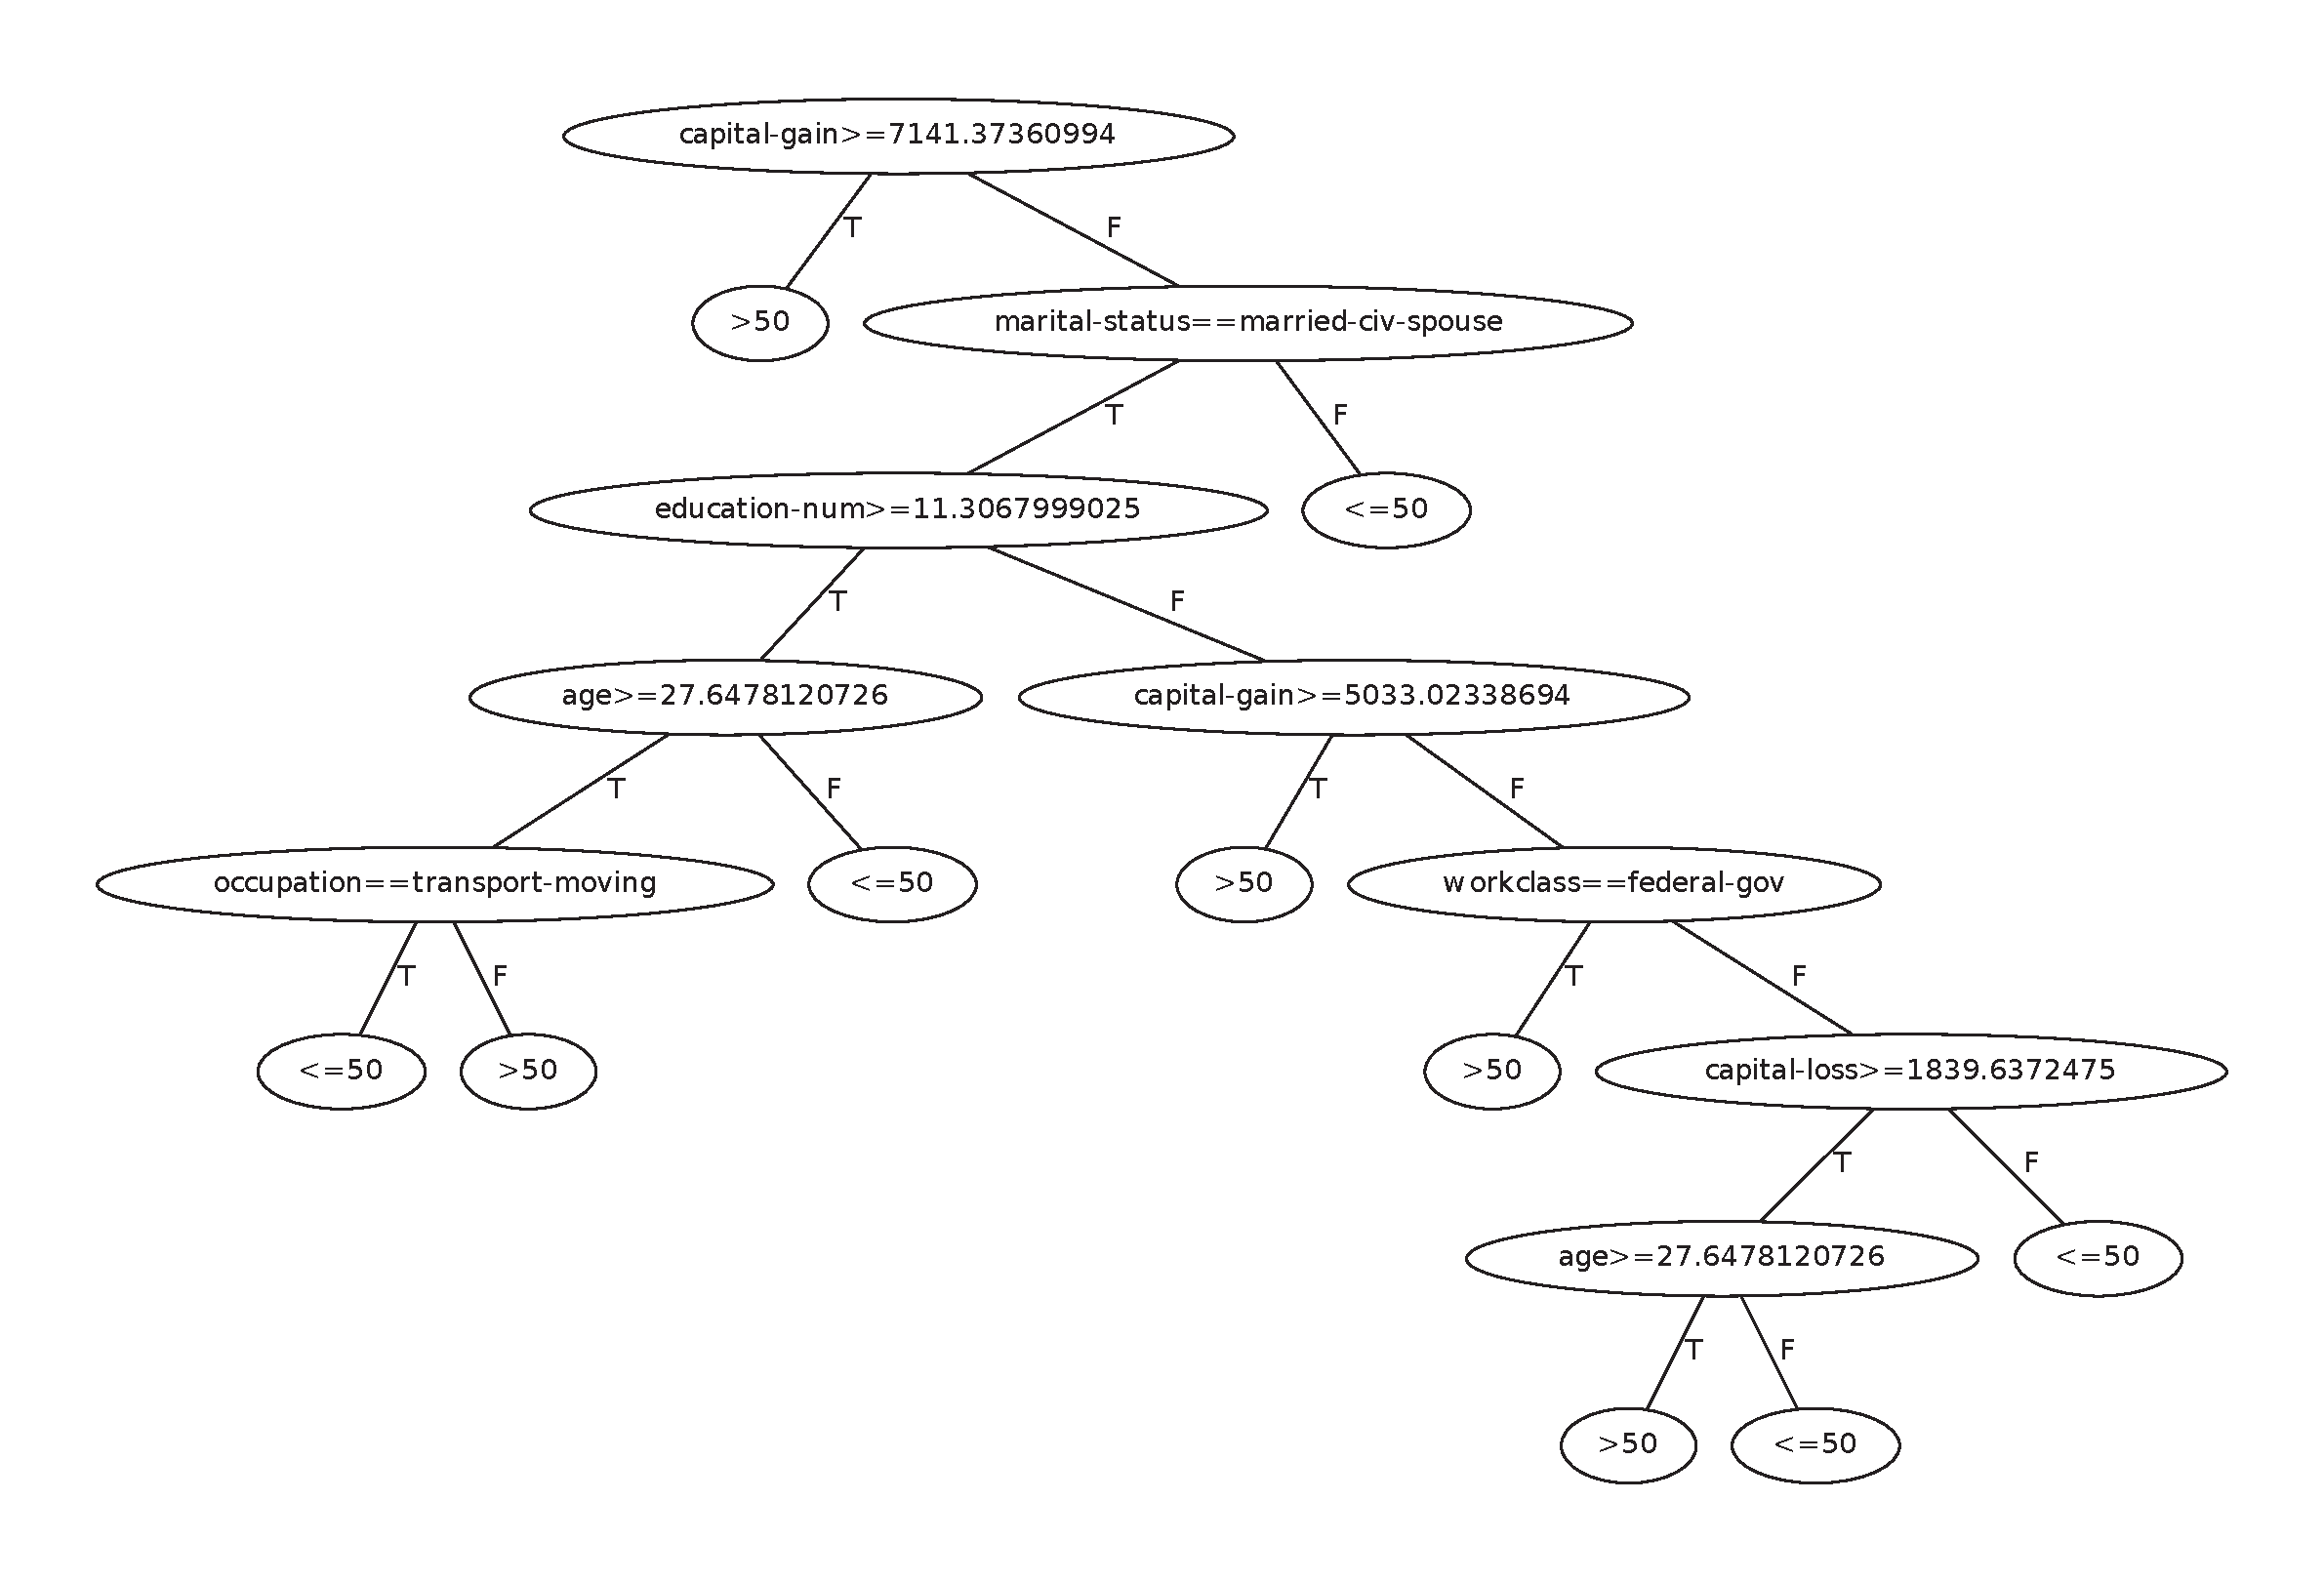
\includegraphics[width=\linewidth]{tree.eps}
\caption{A tree generated by our Pareto ESA algorithm.}\label{tree}
\end{figure*}

We have included a sample tree, in \hyperref[tree]{Figure 1} created by one run of our Pareto ESA algorithm. This very small tree is size 19, yet outperforms the tree created by C4.5 (size 173) on the test set. Interestingly, the first two splits of our example tree consider the same attributes as the first two splits C4.5 makes, with similar values being compared.

\subsubsection{Training Error}

\begin{figure*}[h]
\centering
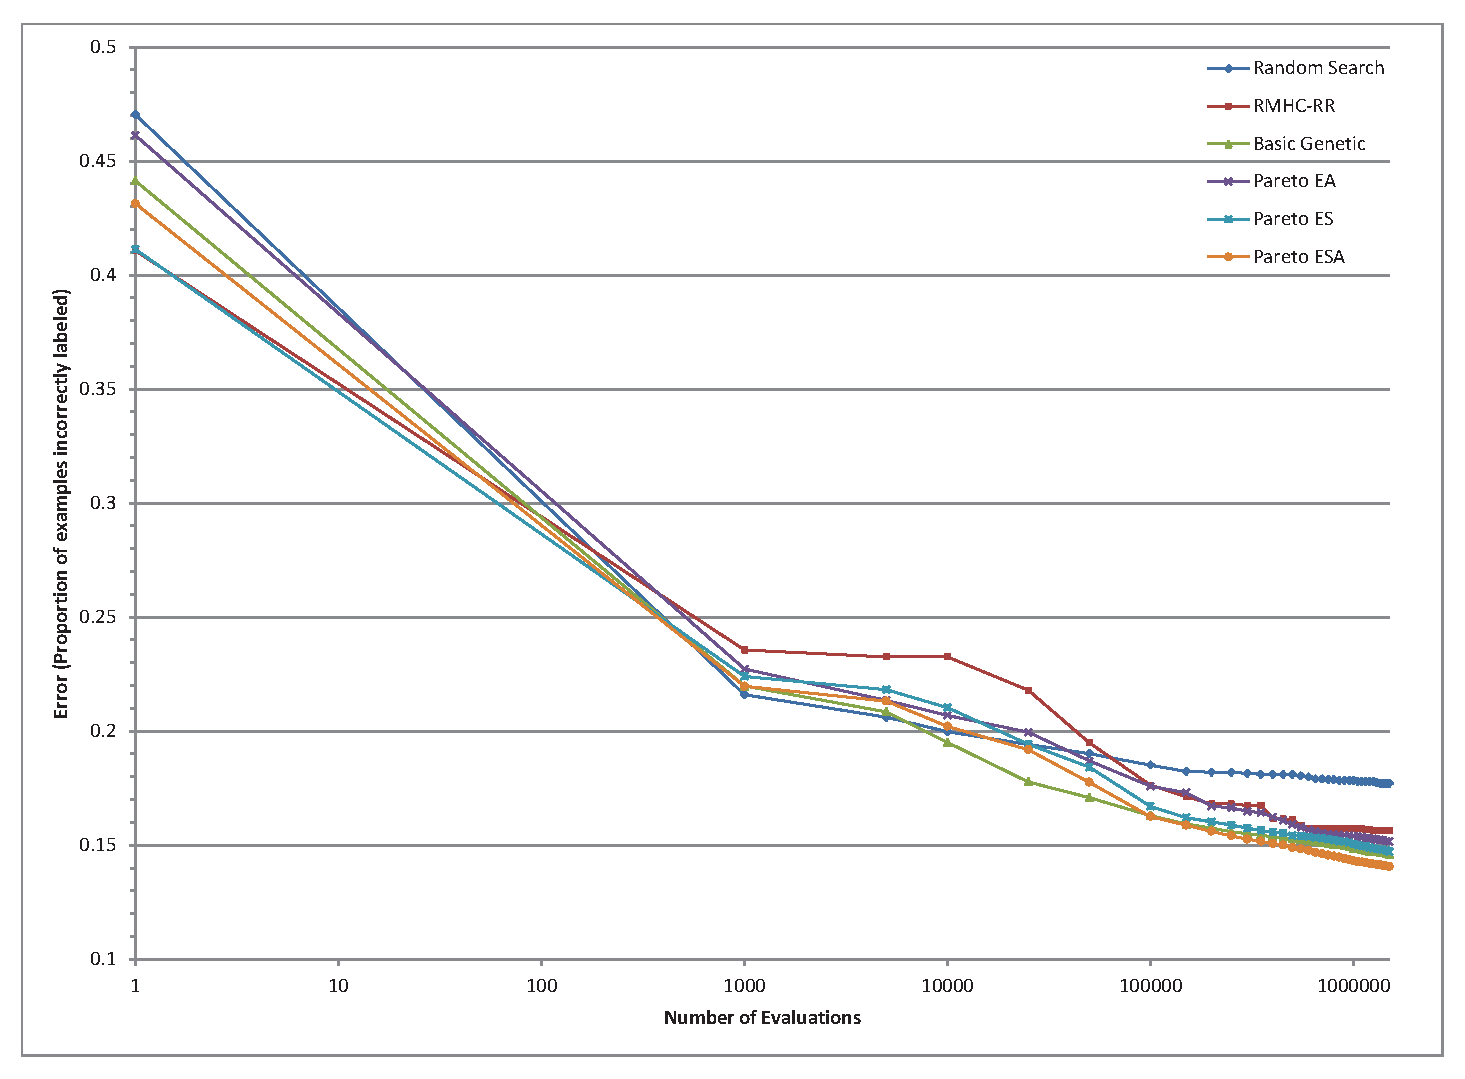
\includegraphics[width=\linewidth]{train_chart.eps}
\caption{Training error vs number of evaluations}\label{train}
\end{figure*}

As can be seen in \hyperref[train]{Figure 2} all of the genetic algorithms outperformed random search and RMHC-RR after about 100,000 evaluations. Pareto ESA was clearly the best, outperforming all other algorithms, while basic genetic and pareto ES were close behind. We did not include error bars in this graph as basic genetic had relatively large standard error and made other error bars unreadable. However, we do include error bars in \hyperref[algorithms]{Figure 4} which shows final train and test error across algorithms.

\subsubsection{Test Error}

\begin{figure*}[h]
\centering
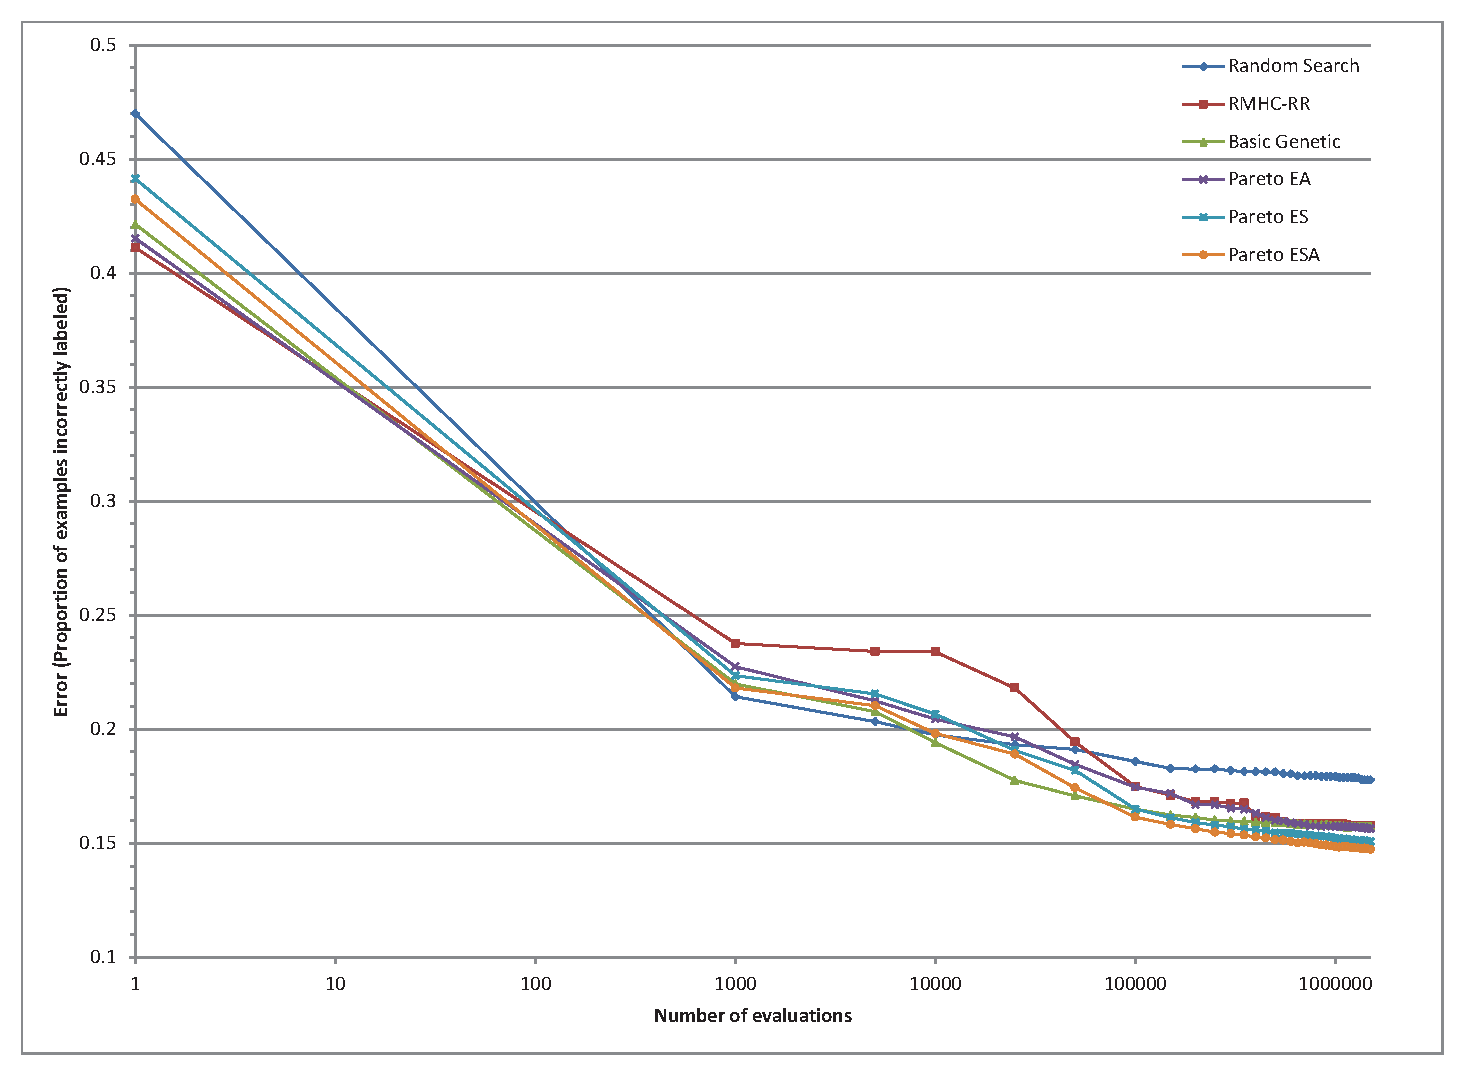
\includegraphics[width=\linewidth]{test_chart.eps}
\caption{Test error vs number of evaluations}\label{test}
\end{figure*}

In terms of test set error, \hyperref[test]{Figure 3}, shows similar results as training error. Pareto ESA is still the best, followed by Pareto ES. However, RMHC-RR begins to catch up basic genetic and pareto EA, though the two genetic algorithms converged faster.

\subsubsection{Error versus Algorithms}

\begin{figure*}[h]
\centering
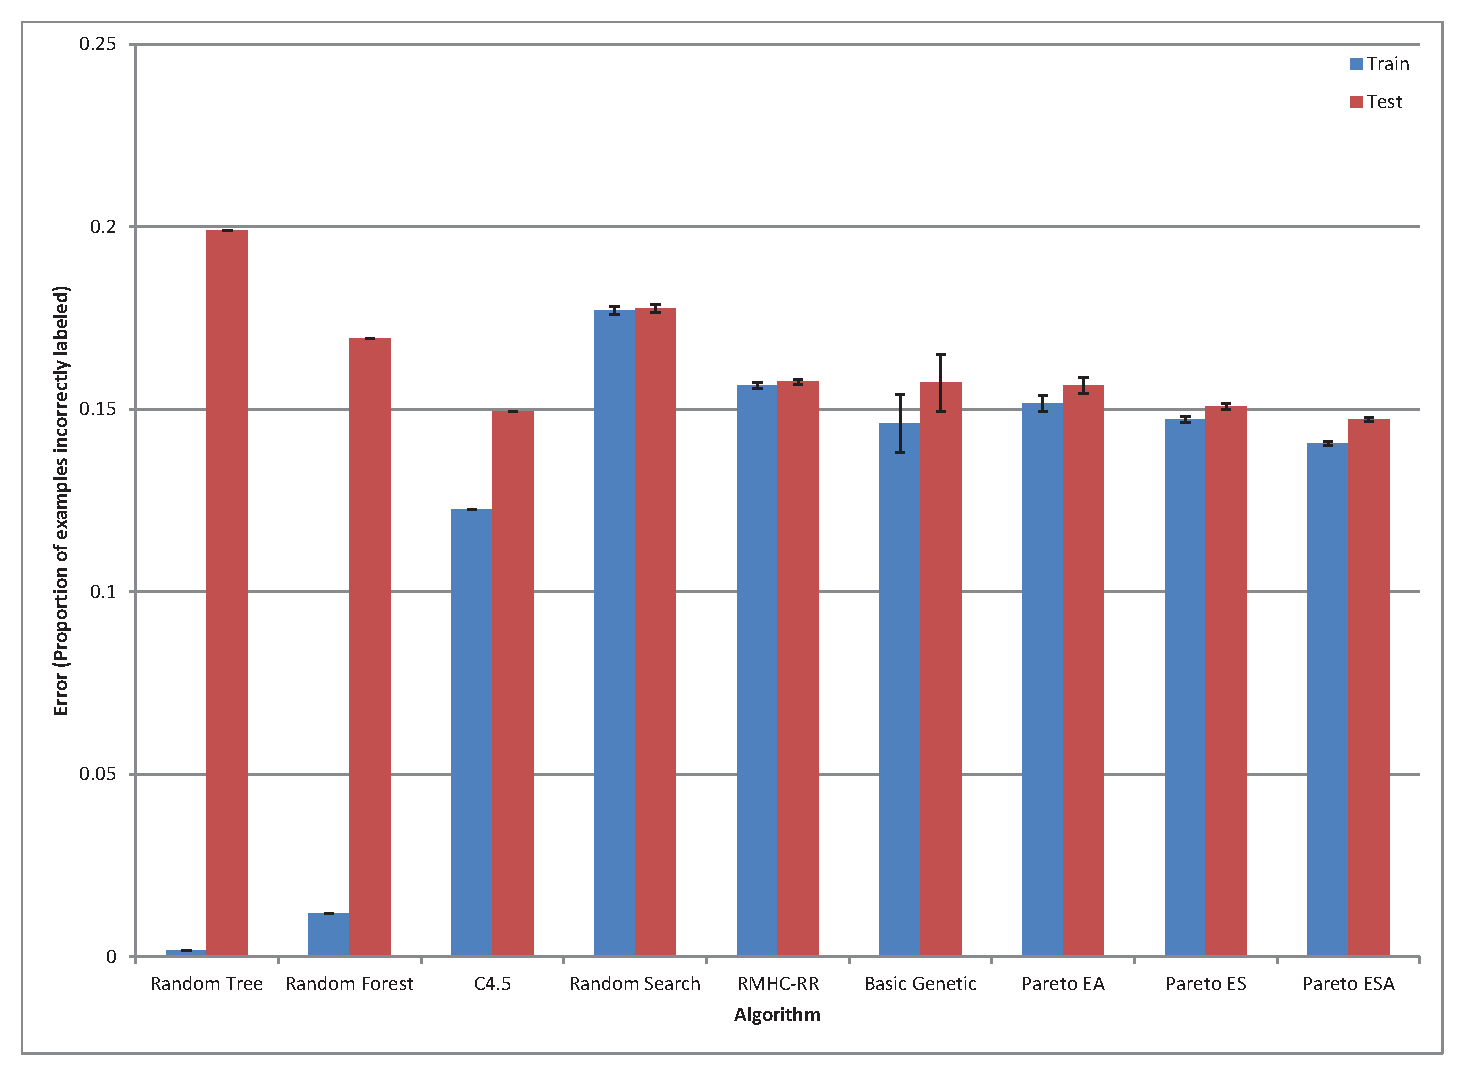
\includegraphics[width=\linewidth]{error_comparison_chart.eps}
\caption{Error comparison across algorithms}\label{algorithms}
\end{figure*}

In \hyperref[algorithms]{Figure 4} we compare how the average train/test error of the final (best) trees from each run of our baseline and genetic algorithms compare to established decision tree algorithms (random tree, random forest and C4.5). As can be seen, Pareto ESA performs the best of any algorithms, being statistically significantly better than C4.5 in terms of the test set. Pareto ES also performs well, though not quite as well as C4.5 in terms of the test set. Pareto EA, basic genetic and RMHC-RR also perform admirably, beating random forest and random tree on average.

\subsubsection{Tree Size}

\begin{figure*}[h]
\centering
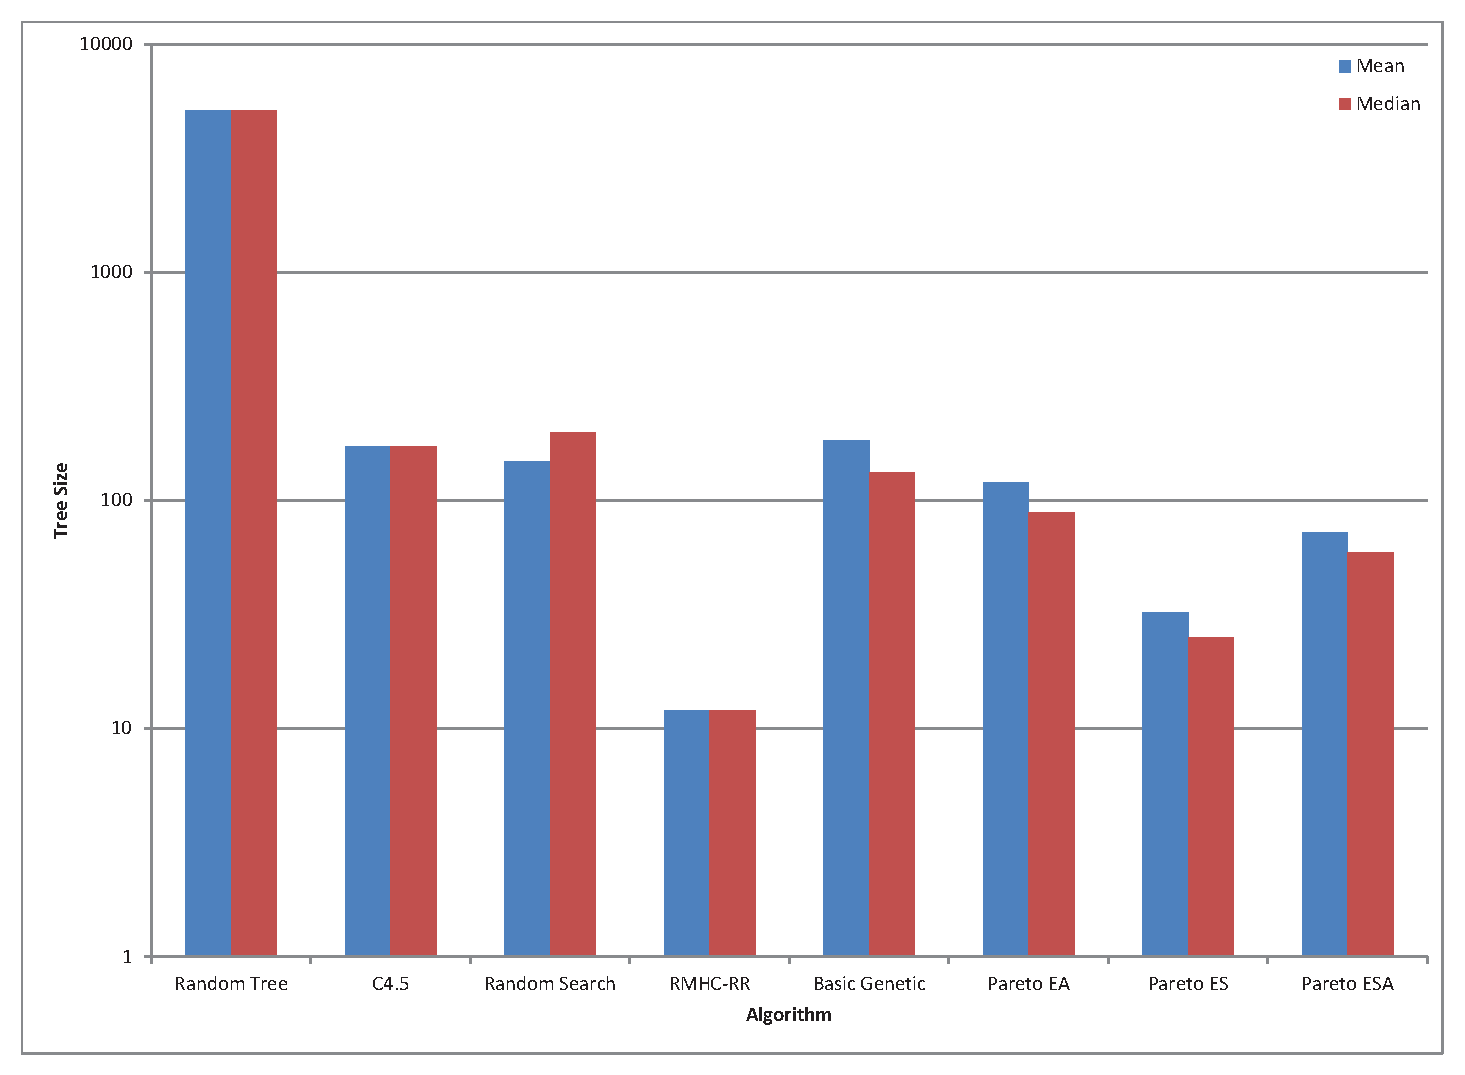
\includegraphics[width=\linewidth]{size_chart.eps}
\caption{Tree size for various algorithms}\label{size}
\end{figure*}

\hyperref[size]{Figure 5}, shows how the average size of the best tree created by each run of our algorithms and baselines as compared to established decision tree algorithms. All our Pareto algorithms created trees that were much smaller than the one created by C4.5 (size 173). In particular Pareto ESA, and Pareto ES produced small trees on average. the tree produced by Weka's \cite{Hall:2009} random tree algorithm was huge, with size over 5000. Basic genetic, creates trees of similar size as C4.5, but slightly larger on average (184 for basic genetic).

\subsubsection{Diversity}

\begin{figure*}[h]
\centering
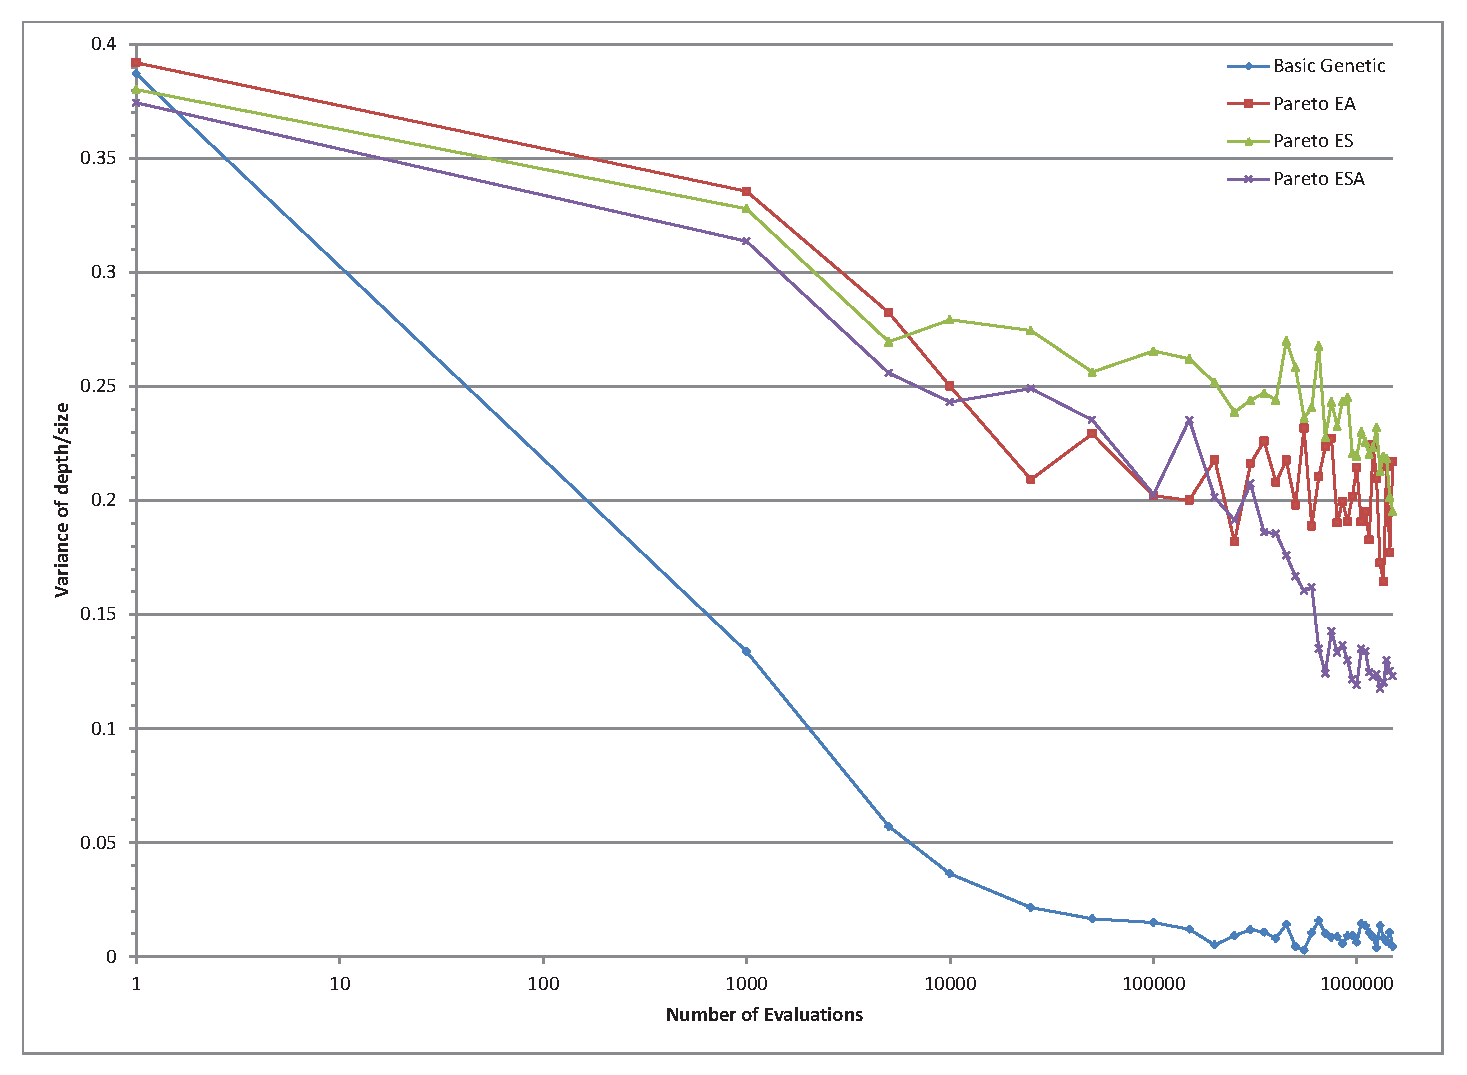
\includegraphics[width=\linewidth]{diversity_chart.eps}
\caption{Diversity measurement vs number of evaluations for our genetic algorithms}\label{diversity}
\end{figure*}

Our Pareto algorithms all maintain diversity much more successfully than our basic genetic algorithm as can be seen in, \hyperref[diversity]{Figure 6}. Pareto ES and pareto EA perform the best in terms of diversity, with pareto ESA performing slightly below them.

\subsection{Discussion}

Our algorithms performed remarkably well, out-performing C4.5, one of the standard algorithms for decision trees (not to mention random forest and random tree), on the test set. Thus our belief that evolutionary algorithms could compete with, and exceed, established algorithms for the induction of decision trees is supported.

Our algorithms, in general, did not outperform the existing algorithms in training error. This may be an indication that our algorithms are overfitting the training data less than existing algorithms because they still performed well on the test data. Overfitting can also be indicated by size of the resulting trees. For instance, random tree creates a tree of over size 5000, and performs extremely well on the training data, but poorly on the test data. Our pareto-based genetic algorithms however tend to produce final trees which are smaller than those of C4.5, random hillclimber and random tree. This indicates that pareto approaches with proper objectives (size and age for instance) allow us to select for smaller, more generalizable trees that do not overfit training data.

Our basic genetic algorithm, however, does not create trees that perform as well consistently. From \hyperref[algorithms]{Figure 4} we can see that basic genetic has a high standard error. This indicates that this algorithm may be too reliant on having specific attributes in the initial population. This problem seems to be relieved in pareto, both because a couple random solutions are included every generation as well as the other objectives (size, age). Basic genetic also seems to be more prone to overfitting than our pareto algorithms as the basic genetic had a larger difference in training and test error, and in general produced larger trees than pareto.

However, both basic genetic and our pareto genetic algorithms performed well, indicating that there are structural patterns within our representation and in decision trees in general that can be exploited via our mutation operators as well as through subtree swapping (our crossover operator) that are not exploited by C4.5 and similar algorithms. C4.5 instead exploits patterns and information within the training data, which may be a reason that there appears to be more overfitting in established algorithms as compared to our algorithms which use the tree structure itself.

In terms of diversity our pareto algorithms easily beat out our basic genetic. We believe this is primarily due to the fact we include a couple new random individuals in each generation which helps maintain a diverse population in our pareto variants. However, including both age and size as objectives in pareto algorithms also are likely to have helped. This is likely because age explicitly selects for younger solutions, thus including solutions closer to age 0 random solutions. Size may also select for solutions that are of variant $\frac{depth}{size}$ because size is a factor in how we determine this diversity score.

\section{Future Work}
An easy way to improve our current algorithms would be parameter tuning. Different mutation rates could be tested or even made variable through the algrithm run, as could crossover rates. Different selection operators (i.e. using a crowding analysis on the pareto layers) would also likely improve convergence.

We spent time working on a variation of our basic genetic algorithm that performs co-evolution on the data used for fitness evaluation. We tried several techniques in which fitness of samples was the average accuracy of trees on the sample (minimizing accuracy) as well as the variance in the accuracy of trees on the sample. We did not have success with either approach so did not include the results in this paper; however, we still believe co-evolution is a promising area for improving our algorithms.

A second area we are looking into is extending our algorithms to generate forests, either through some subset of the population or by accumulating dissimilar trees over the course of the algorithm run and then using this resulting forest to increase performance on test data. This may be particularly applicable to pareto front versions of our algorithms that use the best overall pareto front as the final forest, or some subset of the front.

Finally, using a larger variety of data sets to compare our algorithms to C4.5 and random searches would clarify the performance differences and advantages of each method. Especially on difficult to classify data with error rates nearer $\frac{1}{2}$, we expect a genetic algorithm could outperform C4.5 and related algorithms because it searches through a much larger range of the solution space.

\section{Conclusion}

On the adult data set, our Pareto ESA algorithm outperformed all baselines and established algorithms (in particular, C4.5). Not only did it have lower test error but it created a significantly smaller tree and avoided overfitting the training data to the extent of other algorithms. This emphasizes the advantages of including a Pareto strategy into a genetic algorithm to maintain diversity and develop multiple approaches to the same problem. More generally, the results demonstrate the ability of genetic programming to construct accurate, generalizable decision trees.

While our algorithms could use some optimization and parameter tuning, there were no major failures of the Pareto approach. In creating a solution superior to C4.5 in every metric, the Pareto ESA certainly surpassed expectations.

Since our Pareto ESA algorithm tends to create much smaller trees than C4.5, it actually runs significantly faster on the test data. Given slightly superior error, once created our genetic trees will work much more quickly and more accurately than a C4.5 solution on a large data set. Harder problems might increase this difference. Thus, our results demonstrate the utility of a genetic programming approach to decision tree induction and may spur further investigation into these types of problems.

\section{Acknowledgements}

We would like to acknowledge Professor Hod Lipson, who provided guidance and advice on this project. We would also like to note that we used the Python package, numpy, for much of our computation and the graphing package, Dot, to produce visualizations of our trees.

\section{Appendix}

\begin{tabular}{|l|l|}
\hline
utils.py & Contains our utility, mutation, crossover, fitness and selection functions. \\
baseline.py & Contains our baseline algorithms, random search and RMHC-RR. \\
genetic.py & Contains our genetic algorithms, pareto and basic genetic. \\
run\_algorithms.py & Contains code used for our test harness and data recording. \\
process\_data.py & Contains code used for processing recorded data and computing statistics. \\ \hline
\end{tabular}

%
% The following two commands are all you need in the
% initial runs of your .tex file to
% produce the bibliography for the citations in your paper.
\bibliographystyle{abbrv}
\bibliography{sigproc}  % sigproc.bib is the name of the Bibliography in this case
% You must have a proper ".bib" file
%  and remember to run:
% latex bibtex latex latex
% to resolve all references
%
% ACM needs 'a single self-contained file'!
%
\balancecolumns
% That's all folks!
\end{document}
